\documentclass{article}
\usepackage{amsmath}
\usepackage{amssymb}
\usepackage{graphicx}
\usepackage{hyperref}
\usepackage[version=4]{mhchem}


\begin{document}
(1989 China Middle School Math Contest) As shown in the figure, the area of square \(A B C D\) is \(1989 \mathrm{~cm}^{2} . O\) is the center, \(P\) is a point inside \(A B C D . \angle O P B=45^{\circ} . P A: P B=5: 14\). Find the length of \(P B\).

Solution: 42.\\
\centering
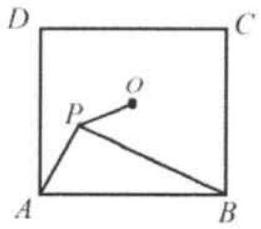
\includegraphics[width=\textwidth]{images/204(2).jpg}

Connect \(O A, O B\).\\
Since \(\angle O P B=\angle O A B=45^{\circ}\), points \(A, B, O\), and \(P\) are concyclic.\\
So \(\angle A P B=\angle A O B=90^{\circ}\).


Let \(P A=5 x, P B=14 x\).\\
Applying Pythagorean Theorem to right triangle \(A P B\) :\\
\((5 x)^{2}+(14 x)^{2}=1989 \Rightarrow \quad x=3\) and \(P B=42\).\\
\centering
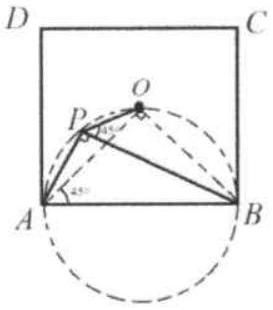
\includegraphics[width=\textwidth]{images/205.jpg}
\end{document}
